\chapter{معادلات ماكسويل، والتغاير، والموجات الكهرومغناطيسية}

\lectureoverview{تؤثر المجالات الكهربائية والمغناطيسية في المادة المشحونة عبر قوة لورنتز، لكن لا بد أيضًا أن تُنشئ المادة هذه المجالات وأن تعيد ترتيبها. سنصوغ ذلك النصف المتبادل من الكهرومغناطيسية، ونبيّن أن معادلات ماكسويل متغايرة لورنتزيًا، ونشتق حلولها الموجية، ثم نعيد إدخال الشحنة والتيار بصيغة تجعل الانحفاظ الموضعي ظاهرًا بجلاء. وطوال هذه المحاضرة نستخدم وحدات يكون فيها \(c=1\).}

\section{النصف الآخر من الكهرومغناطيسية}

لنبدأ بالجزء الذي صار بين أيدينا من الموضوع. إذا تحرك جسيم شحنته \(q\) بسرعة \(\mathbf v\) عبر مجالين كهربائي ومغناطيسي، فإن القوة هي
\begin{equation}
\mathbf F=q\bigl(\mathbf E+\mathbf v\times\mathbf B\bigr).
\label{eq:lorentz-force-three}
\end{equation}
إن العامل \(q\) لا غنى عنه. فالجسيم غير المشحون لا يتأثر بالقوة الكهرومغناطيسية. ويسهم المجال الكهربائي حتى عندما يكون الجسيم ساكنًا آنيًا، في حين تعتمد المساهمة المغناطيسية على حركته.

تخبرنا المعادلة~\eqref{eq:lorentz-force-three} بما تفعله المجالات المعطاة بالمادة. لكنها لا تخبرنا بما يحدد المجالات نفسها. ما الذي يولد مجالًا كهربائيًا حول جسم، ومجالًا مغناطيسيًا حول آخر، أو موجةً تتحرك عبر الفضاء الخالي؟ المعادلات التي تجيب عن هذه الأسئلة هي معادلات ماكسويل.

\begin{figure}[H]
\centering
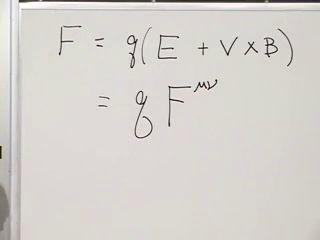
\includegraphics[width=0.62\textwidth]{lecture_58_figure_02.png}
\caption{قوة لورنتز بصيغة المتجه الثلاثي وبداية إعادة صياغتها الموترية.}
\lectureframe{00:05:49}
\end{figure}

تستبق الصيغة النسبية لقانون القوة الترميز الذي سنحتاج إليه:
\begin{equation}
f^\mu=qF^\mu{}_{\nu}u^\nu.
\label{eq:lorentz-force-four}
\end{equation}
هنا \(u^\nu\) هو السرعة الرباعية، و\(f^\mu\) هو القوة الرباعية، و\(F^{\mu\nu}\) موتر مضاد للتماثل مُركَّب من \(\mathbf E\) و\(\mathbf B\). ويعرض اللوح أولًا مجرد بداية تخطيطية لهذا التعبير؛ ويزوّدنا الانكماش مع \(u^\nu\) بالمتجه المفقود اللازم لترك فهرس قوة واحد حرًا.

هناك سبب فيزيائي يقتضي أن تؤثر المادة بدورها في المجال. فبإمكان موجة كهرومغناطيسية أن تصطدم بشحنة، فتسرّعها وتنقل إليها طاقة. ولو كان المجال يستطيع التأثير في الشحنة بينما لا تستطيع الشحنة قط التأثير في المجال، لما وُجد موضع سُحبت منه تلك الطاقة. وليس الفعل ورد الفعل تمام الحجة كلها، لكن انحفاظ الطاقة يجعل الاقتران المتبادل أمرًا لا مفر منه.

\section{مصدر متغير يبعث اضطرابًا}

تنتج الشحنة النقطية مجالًا كهربائيًا يتجه إلى الخارج من موضعها أو إلى داخله. وينتج تيار في سلك--أي تدفق جسيمات مشحونة--مجالًا مغناطيسيًا يدور حول السلك. وهذه الصور الساكنة المألوفة تُظهر بالفعل نمطين هندسيين مختلفين: فالفيض الكهربائي ينبعث من الشحنة، بينما تلتف خطوط المجال المغناطيسي حول التيار.

والآن حرّك الشحنة النقطية فجأة. بالقرب من موضعها الجديد لا بد أن يبدأ المجال الكهربائي بإعادة ترتيب نفسه، لكن مراقبًا بعيدًا لا يستطيع أن يعلم بالحركة على الفور. ويبقى المجال القديم بعيدًا إلى أن تتاح لإشارة فرصة الوصول. وبين المنطقتين القريبة والبعيدة تقع جبهة متحركة يتغير عندها المجال. وهذه إعادة الترتيب المتحركة هي اضطراب كهرومغناطيسي.

إذا أُجبرت الشحنة على الحركة ذهابًا وإيابًا، فإن عمليات إعادة ترتيب متعاقبة تتلو بعضها بعضًا وتشكّل موجة كهرومغناطيسية. وهذه هي الوظيفة الأولية للهوائي: تيار كهربائي متذبذب يبعث اضطرابًا في المجال إلى الخارج. ويعطي عكس تيار في سلك النسخة المغناطيسية من الحجة نفسها. فلا بد أن ينعكس دوران \(\mathbf B\)، لكن هذا الانعكاس ينتشر بدلًا من أن يظهر في كل مكان دفعة واحدة.

تضع هذه الصورة السببية هدفين لمعادلات ماكسويل. فلا بد أن تصف كيف تكون الشحنة والتيار مصدرين للمجالات، ولا بد أن تسمح بأن تنتشر التغيرات في تلك المجالات بسرعة لا تتجاوز سرعة الضوء. والهدف الثاني هو أيضًا اختبار للنسبية. فإذا كانت معادلات ماكسويل تأخذ الصيغة نفسها في كل إطار قصوري وتستلزم سرعة موجية محددة، فلا بد أن يستنتج كل إطار قصوري السرعة نفسها منها.

\section{مراجعة معادلة الموجة النسبية}

قبل الانتقال إلى المجالات المتجهية، تأمل مجالًا قياسيًا \(\phi(\mathbf x,t)\)، أي عددًا واحدًا عند كل نقطة من الزمكان. إن معادلة من الرتبة الأولى
\begin{equation}
\partial_\mu\phi=0
\end{equation}
كانت لتقول إن كل مشتقة زمكانية تنعدم. وعندئذ يكون المجال ثابتًا، ومن ثم غير قادر على حمل موجة. أما معادلة موجة نسبية غير تافهة فتستخدم مشتقتين:
\begin{equation}
\partial_\mu\partial^\mu\phi=0.
\end{equation}
ومع اصطلاح الإشارة المستخدم هنا،
\begin{equation}
\left(\partial_t^2-\partial_x^2-\partial_y^2-\partial_z^2\right)\phi=0,
\label{eq:scalar-wave-four}
\end{equation}
أو، بصورة أكثر اختصارًا،
\begin{equation}
\left(\partial_t^2-\nabla^2\right)\phi=0.
\end{equation}
ويجعل الاختيار \(c=1\) الزمن والمسافة يحملان وحدات متوافقة. وإذا أعدنا الوحدات المعتادة فسيظهر \(1/c^2\) إلى جانب المشتقة الزمنية الثانية.

بالنسبة إلى موجة تسير على طول المحور \(z\)، يعتمد المجال على \(z\) و\(t\)، لا على \(x\) أو \(y\). وتُختزل المعادلة~\eqref{eq:scalar-wave-four} إلى
\begin{equation}
\left(\partial_t^2-\partial_z^2\right)\phi=0.
\label{eq:scalar-wave-one}
\end{equation}

\begin{figure}[H]
\centering
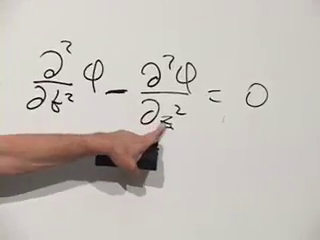
\includegraphics[width=0.56\textwidth]{lecture_58_figure_04.png}
\caption{معادلة الموجة القياسية أحادية البعد المستخدمة نموذجًا للموجات الكهرومغناطيسية.}
\lectureframe{00:47:03}
\end{figure}

وصيغتها العامة لموجة منتقلة هي
\begin{equation}
\phi(z,t)=f(z-t)+g(z+t).
\end{equation}
تتحرك الهيئة \(f(z-t)\) نحو تزايد \(z\)، لأن نقطة ذات طور ثابت تحقق \(z-t=\text{constant}\). أما الهيئة \(g(z+t)\) فتتحرك في الاتجاه المعاكس. ولا شيء يفرض أن تكون أي من الهيئتين جيبية؛ فأي شكل أملس بما يكفي ينتقل من غير أن يغيّر شكله.

ومع ذلك تبقى الدوال الجيبية ملائمة:
\begin{equation}
\phi(z,t)=A\cos\!\bigl(k(z-t)\bigr).
\end{equation}
ويتحكم عدد الموجة \(k\) في الطول الموجي،
\begin{equation}
\lambda=\frac{2\pi}{k}.
\end{equation}
فالقيمة الكبيرة لـ\(k\) تولّد تذبذبًا مكانيًا سريعًا وطولًا موجيًا قصيرًا؛ أما القيمة الصغيرة لـ\(k\) فتولّد طولًا موجيًا طويلًا. وهذه الهيئات نفسها ستصبح بعد قليل مركبات \(\mathbf E\) و\(\mathbf B\).

\section{حساب المتجهات الذي تحتاج إليه معادلات ماكسويل}

تُكتب معادلات ماكسويل باستخدام الجداء النقطي، والجداء الاتجاهي، والتباعد، والدوران. ويستحق الأمر أن نعيد بناء هذا الترميز مرة واحدة، لأن حسابات المركبات اللاحقة تستخدم هذه الأنماط نفسها على وجه الدقة.

بالنسبة إلى المتجهين الثلاثيين العاديين \(\mathbf a\) و\(\mathbf b\)، فالجداء النقطي هو الكمية القياسية
\begin{equation}
\mathbf a\cdot\mathbf b
=a_xb_x+a_yb_y+a_zb_z.
\end{equation}
أما الجداء الاتجاهي فهو متجه آخر،
\begin{align}
(\mathbf a\times\mathbf b)_x&=a_yb_z-a_zb_y,\\
(\mathbf a\times\mathbf b)_y&=a_zb_x-a_xb_z,\\
(\mathbf a\times\mathbf b)_z&=a_xb_y-a_yb_x.
\end{align}
وتتبع المركبات الباقية من الترتيب الدوري \(x\to y\to z\to x\).

لنعرّف المؤثر التفاضلي
\begin{equation}
\boldsymbol\nabla=
\left(\partial_x,\partial_y,\partial_z\right).
\end{equation}
فمدخلاته مؤثرات لا أعداد عادية، لكن لا يزال بالإمكان استخدام نمطي الجداء النقطي والاتجاهي. وبالنسبة إلى مجال متجهي \(\mathbf A\)، فإن
\begin{equation}
\boldsymbol\nabla\cdot\mathbf A
=\partial_xA_x+\partial_yA_y+\partial_zA_z
\label{eq:divergence}
\end{equation}
هو التباعد، بينما
\begin{align}
(\boldsymbol\nabla\times\mathbf A)_x
 &=\partial_yA_z-\partial_zA_y,\\
(\boldsymbol\nabla\times\mathbf A)_y
 &=\partial_zA_x-\partial_xA_z,\\
(\boldsymbol\nabla\times\mathbf A)_z
 &=\partial_xA_y-\partial_yA_x
\label{eq:curl}
\end{align}
هي مركبات الدوران.

الهندسة لا تقل أهمية عن الصيغ. يكون للمجال المتجهي تباعد موجب حيث يبدو أنه يتدفق إلى الخارج من مصدر. ويكون له دوران حيث يدور. ويجسّد المجال الكهربائي الشعاعي لشحنة نقطية التباعد؛ ويجسّد المجال المغناطيسي الملتف حول سلك يحمل تيارًا الدوران. أما المجال المتجهي الثابت مكانيًا فلا يملك أيًا منهما.

\section{معادلات ماكسويل في الفراغ}

في غياب الشحنة والتيار، تكون معادلات ماكسويل هي
\begin{align}
\boldsymbol\nabla\times\mathbf E&=-\partial_t\mathbf B,
\label{eq:faraday-vac}\\
\boldsymbol\nabla\cdot\mathbf B&=0,
\label{eq:gauss-b-vac}\\
\boldsymbol\nabla\times\mathbf B&=\partial_t\mathbf E,
\label{eq:ampere-vac}\\
\boldsymbol\nabla\cdot\mathbf E&=0.
\label{eq:gauss-e-vac}
\end{align}
تكاد معادلتا الدوران أن تتبادلا \(\mathbf E\) و\(\mathbf B\)، لكن إشارة سالب أساسية تميّزهما. وتقول معادلتا التباعد إن أيًا من المجالين لا يملك مصدرًا في منطقة الفراغ موضع النظر. ويظل تباعد المجال المغناطيسي صفرًا حتى بعد إعادة المصادر الكهربائية؛ فالكهرومغناطيسية العادية لا تتضمن شحنة مغناطيسية.

\begin{figure}[H]
\centering
\includegraphics[width=0.76\textwidth]{lecture_58_figure_06.png}
\caption{معادلات ماكسويل الأربع في الفراغ، مرتبة لإظهار التناظر القريب بين المجالين الكهربائي والمغناطيسي.}
\lectureframe{00:27:30}
\end{figure}

ستحل كثافة الشحنة \(\rho\) في النهاية محل الصفر على الطرف الأيمن من المعادلة~\eqref{eq:gauss-e-vac}، وستدخل كثافة التيار \(\mathbf J\) في المعادلة~\eqref{eq:ampere-vac}. ونؤجل هذين الحدين مؤقتًا. فالمعادلات الخالية من المصدر تكشف بنية التحول وآلية الموجة بأقل قدر من التشويش.

كما أنها تزيد أحجية أينشتاين حدّة. فالمراقب الغاليلي الذي يتبع موجة سيتوقع أن يطرح السرعات وأن يقيس سرعة موجية أصغر. ومع ذلك، إذا كانت معادلات ماكسويل نفسها تصح في كل إطار قصوري، فإن كل مراقب يستنبط منها السرعة الموجية الوحدوية نفسها. وليس المخرج هو تغيير معادلة الموجة من إطار إلى إطار، بل استخدام تحويل لورنتز وإظهار معادلات ماكسويل على هيئة كميات صارت قوانين تحولها معروفة سلفًا.

\section{المجالان الكهربائي والمغناطيسي بوصفهما موترًا واحدًا}

يتحد المجالان الكهربائي والمغناطيسي في موتر المجال المضاد للتماثل
\begin{equation}
F^{\mu\nu}=
\begin{pmatrix}
0   & -E_x & -E_y & -E_z\\
E_x & 0    & -B_z & B_y\\
E_y & B_z  & 0    & -B_x\\
E_z & -B_y & B_x  & 0
\end{pmatrix},
\label{eq:l0203-field-tensor}
\end{equation}
حيث ترتيب الصفوف والأعمدة هو \(t,x,y,z\). ويفرض التضاد في التماثل،
\begin{equation}
F^{\mu\nu}=-F^{\nu\mu},
\end{equation}
أن تنعدم العناصر القطرية وأن يُحدَّد النصف السفلي من المصفوفة من نصفها العلوي. وتحتوي العناصر المختلطة زمانًا ومكانًا على \(\mathbf E\)؛ أما العناصر المكانية الخالصة فتحتوي على \(\mathbf B\).

\begin{figure}[H]
\centering
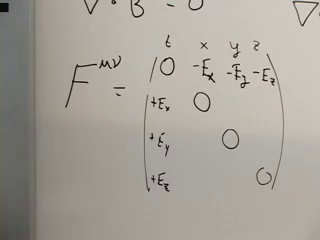
\includegraphics[width=0.58\textwidth]{lecture_58_figure_03.png}
\caption{موتر المجال الكهرومغناطيسي المكتمل، بما في ذلك عناصره الكهربائية والمغناطيسية.}
\lectureframe{00:32:05}
\end{figure}

ليست أهمية \(F^{\mu\nu}\) مجرد أن مركبات المجال الست تنتظم في مصفوفة واحدة. فعند تحويل لورنتز يتحول كموتر من الرتبة الثانية. ولذلك يختلط المجالان الكهربائي والمغناطيسي كما يقيسهما مراقبون مختلفون على النحو المطلوب تمامًا لكي يتحول الكل تحوّلًا متسقًا.

يوجد موترٌ مضادّ التناظر ثانٍ، هو موتر المجال المزدوج \(\widetilde F^{\mu\nu}\). ووفق الاصطلاح المعتمد هنا يُحصَل عليه من المعادلة~\eqref{eq:l0203-field-tensor} بالاستبدال
\begin{equation}
\mathbf E\longmapsto-\mathbf B,
\qquad
\mathbf B\longmapsto\mathbf E.
\label{eq:dual-replacement}
\end{equation}
ومن ثم
\begin{equation}
\widetilde F^{\mu\nu}=
\begin{pmatrix}
0    & B_x  & B_y  & B_z\\
-B_x & 0    & -E_z & E_y\\
-B_y & E_z  & 0    & -E_x\\
-B_z & -E_y & E_x  & 0
\end{pmatrix}.
\label{eq:dual-tensor}
\end{equation}
إن الإشارة في المعادلة~\eqref{eq:dual-replacement} مهمة. تبدأ المحاضرة أولًا بمحاولة هذا التبديل شفهيًا، ثم تلتقط عدم تطابق الإشارة وتصححه قبل إكمال المصفوفة.

\begin{figure}[H]
\centering
\includegraphics[width=0.58\textwidth]{lecture_58_figure_07.png}
\caption{تجميع الموتر المزدوج بتبديل المدخلات الكهربائية والمغناطيسية مع الإشارة المطلوبة.}
\lectureframe{00:35:45}
\end{figure}

\section{معادلات الفراغ التغايرية}

تحتوي كل معادلة من معادلات ماكسويل على مشتقة واحدة. والبدء من موتر من الرتبة الثانية ثم إجراء انكماش مع أحد فهارس المشتقة يترك فهرسًا حرًا واحدًا، لذا فإن المرشحين التغايريين الطبيعيين هما
\begin{align}
\partial_\mu F^{\mu\nu}&=0,
\label{eq:maxwell-covariant-vac}\\
\partial_\mu\widetilde F^{\mu\nu}&=0.
\label{eq:maxwell-dual-vac}
\end{align}
ولكل قيمة ثابتة لـ \(\nu\)، تكون المعادلة~\eqref{eq:maxwell-covariant-vac} معادلة واحدة. وبما أن \(\nu\) يمكن أن تكون \(t,x,y,z\)، فهي تجمع أربع معادلات قياسية. والمعادلة~\eqref{eq:maxwell-dual-vac} تجمع الأربع الأخرى. وهذا يطابق معادلتي الدوران المتجهيتين ومعادلتي التباعد القياسيتين في القائمة الأصلية.

لا تكون الصياغة المختصرة مفيدة إلا إذا أعادت إنتاج المعادلات المألوفة. خذ \(\nu=z\):
\begin{align}
\partial_\mu F^{\mu z}
&=\partial_tF^{tz}
  +\partial_xF^{xz}
  +\partial_yF^{yz}
  +\partial_zF^{zz}\\
&=-\partial_tE_z+\partial_xB_y-\partial_yB_x\\
&=-\partial_tE_z+
  \bigl(\boldsymbol\nabla\times\mathbf B\bigr)_z.
\end{align}
ينعدم الحد \(F^{zz}\) بسبب مضادّة التناظر. وجعل النتيجة مساوية للصفر يعطي المركبة \(z\) من
\begin{equation}
\boldsymbol\nabla\times\mathbf B=\partial_t\mathbf E.
\end{equation}
وتنتج المركبتان \(x\) و\(y\) بالتدوير الدوري للفهارس.

\begin{figure}[H]
\centering
\includegraphics[width=0.76\textwidth]{lecture_58_figure_08.png}
\caption{التوسّع بالمركبات للمعادلة التغايرية للمجال؛ المدخل القطري للموتر ينعدم، وتعيد الحدود المتبقية بناء معادلات ماكسويل.}
\lectureframe{00:43:30}
\end{figure}

والآن خذ المركبة الزمنية:
\begin{align}
\partial_\mu F^{\mu t}
&=\partial_tF^{tt}
  +\partial_xF^{xt}
  +\partial_yF^{yt}
  +\partial_zF^{zt}\\
&=\partial_xE_x+\partial_yE_y+\partial_zE_z\\
&=\boldsymbol\nabla\cdot\mathbf E.
\end{align}
ولذلك فهي تعطي المعادلة~\eqref{eq:gauss-e-vac}. ويؤدي إجراء الفحوص نفسها على الموتر المزدوج إلى
\(\boldsymbol\nabla\cdot\mathbf B=0\) و
\(\boldsymbol\nabla\times\mathbf E=-\partial_t\mathbf B\).

أصبحت المعادلات المختصرة الآن مُثبتة لا مجرد مخمَّنة. وبنية فهارسها الحرة تجعلها معادلات رباعية المتجه، لذا فإن تحويل لورنتز يغيّر مركباتها لا شكلها. وهذا هو المعنى الدقيق الذي تكون به معادلات ماكسويل في الفراغ هي نفسها في كل إطار قصوري.

\section{من معادلات من الرتبة الأولى إلى موجة}

تتضمن معادلات ماكسويل مشتقات أولى فقط، في حين تتضمن المعادلة الموجية مشتقات ثانية. ويزول هذا التعارض الظاهري لأن نظرية ماكسويل تقرن بين مجالين. ويمكن جمع زوج من المعادلات من الرتبة الأولى لـ \(\mathbf E\) و\(\mathbf B\) في معادلة من الرتبة الثانية لأيٍّ من المجالين على حدة.

اشتق المعادلة~\eqref{eq:ampere-vac} بالنسبة إلى الزمن:
\begin{equation}
\partial_t^2\mathbf E
=\boldsymbol\nabla\times\partial_t\mathbf B.
\end{equation}
ويوفّر قانون فاراداي المشتقة الزمنية لـ \(\mathbf B\)،
\begin{equation}
\partial_t\mathbf B=-\boldsymbol\nabla\times\mathbf E,
\end{equation}
ومن ثم
\begin{equation}
\partial_t^2\mathbf E
=-\boldsymbol\nabla\times
  \bigl(\boldsymbol\nabla\times\mathbf E\bigr).
\label{eq:double-curl}
\end{equation}

تستعرض السبورة حساب مركبة واحدة بدلًا من استدعاء متطابقة محفوظة. بالنسبة إلى المركبة \(x\)،
\begin{align}
\bigl[\boldsymbol\nabla\times
(\boldsymbol\nabla\times\mathbf E)\bigr]_x
&=\partial_y(\boldsymbol\nabla\times\mathbf E)_z
 -\partial_z(\boldsymbol\nabla\times\mathbf E)_y\\
&=\partial_y(\partial_xE_y-\partial_yE_x)\\
&\quad-\partial_z(\partial_zE_x-\partial_xE_z)\\
&=\partial_x(\partial_yE_y+\partial_zE_z)
 -\partial_y^2E_x\\
&\quad-\partial_z^2E_x.
\end{align}
أضف واطرح \(\partial_x^2E_x\) لإبراز التباعد:
\begin{align}
\bigl[\boldsymbol\nabla\times
(\boldsymbol\nabla\times\mathbf E)\bigr]_x
&=\partial_x(\boldsymbol\nabla\cdot\mathbf E)
 -\nabla^2E_x.
\label{eq:double-curl-x}
\end{align}
في الفراغ \(\boldsymbol\nabla\cdot\mathbf E=0\). وبضم
المعادلتين~\eqref{eq:double-curl} و\eqref{eq:double-curl-x} نحصل على
\begin{equation}
\left(\partial_t^2-\nabla^2\right)E_x=0.
\label{eq:ex-wave}
\end{equation}

\begin{figure}[H]
\centering
\includegraphics[width=0.72\textwidth]{lecture_58_figure_09.png}
\caption{ينتهي الحساب بالمركبات إلى المعادلة الموجية لـ \(E_x\).}
\lectureframe{00:57:10}
\end{figure}

ينطبق الحساب نفسه على \(E_y\) و\(E_z\)، ويعطي حذف مماثل
\begin{equation}
\left(\partial_t^2-\nabla^2\right)\mathbf B=0.
\end{equation}
ولذلك يمكن للمجالين الكهربائي والمغناطيسي أن ينتشرا عبر الفضاء الخالي على هيئة موجات. وفي الوحدات المستخدمة هنا تكون سرعتهما واحدًا، أي إن السرعة هي \(c\) عند إعادة الوحدات المعتادة.

\section{موجة مستوية واستقطابها}

لننشئ موجة بسيطة تسير في الاتجاه الموجب لـ \(z\):
\begin{equation}
\mathbf E(z,t)
=\widehat{\mathbf x}\,E_0
  \cos\!\bigl(k(z-t)\bigr).
\label{eq:plane-e}
\end{equation}
ينزاح شكلها على طول \(z\) من دون أن يتغير. ولأن المجال الكهربائي يشير على طول محور \(x\)، فالموجة مستقطبة خطيًا في اتجاه \(x\). ولم نختر \(E_y=0\) إلا للإبقاء على المثال بسيطًا؛ إذ يمكن إدراج استقطاب عرضي ثانٍ.

المركبة الطولية ليست حرة بالقدر نفسه. وبما أن الموجة تعتمد فقط على \(z\) و\(t\)،
\begin{equation}
\boldsymbol\nabla\cdot\mathbf E
=\partial_zE_z=0.
\end{equation}
وبالتالي يمكن أن يكون \(E_z\) ثابتًا، لكنه لا يمكن أن يحتوي على الشكل الموجي المتغير. ويمكن تراكب مجال خلفية منتظم أو إزالته بصورة مستقلة؛ فهو ليس جزءًا من الإشعاع المنتشر. أما الموجة نفسها فهي عرضية:
\begin{equation}
\mathbf E_{\mathrm{wave}}\cdot\widehat{\mathbf z}=0.
\end{equation}

يحدد قانون فاراداي المجال المغناطيسي. وبالنسبة إلى المعادلة~\eqref{eq:plane-e}، فإن المركبة غير المنعدمة الوحيدة لـ \(\boldsymbol\nabla\times\mathbf E\) هي المركبة \(y\)،
\begin{equation}
(\boldsymbol\nabla\times\mathbf E)_y=\partial_zE_x.
\end{equation}
ونتيجة لذلك فإن \(\partial_t\mathbf B\) يتجه على طول \(y\)، واختيار متوافق هو
\begin{equation}
\mathbf B(z,t)
=\widehat{\mathbf y}\,E_0
  \cos\!\bigl(k(z-t)\bigr).
\label{eq:plane-b}
\end{equation}
في هذه الوحدات تتساوى سعتا المجالين الكهربائي والمغناطيسي. ويحقق اتجاههما
\begin{equation}
\mathbf E\perp\mathbf B,
\qquad
\mathbf E\perp\widehat{\mathbf z},
\qquad
\mathbf B\perp\widehat{\mathbf z},
\qquad
\mathbf E\times\mathbf B\parallel\widehat{\mathbf z}.
\end{equation}

\begin{figure}[H]
\centering
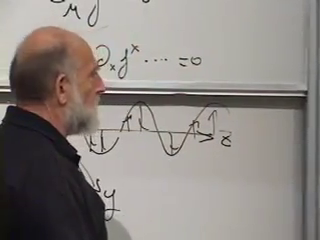
\includegraphics[width=0.70\textwidth]{lecture_58_figure_05.png}
\caption{الرسم التخطيطي المكتمل على السبورة لموجة كهرومغناطيسية عرضية: اهتزازا المجالين الكهربائي والمغناطيسي متعامدان أحدهما على الآخر وعلى اتجاه الانتشار.}
\lectureframe{01:05:25}
\end{figure}

\begin{figure}[H]
\centering
\scalebox{0.90}{%
\begin{tikzpicture}[x=1cm,y=1cm,>=Latex]
  \draw[->,thick] (0,0) -- (8.2,0) node[right] {$z$};
  \draw[->,thick] (0,-1.6) -- (0,1.7) node[above] {$x$};
  \draw[->,thick] (0,0) -- (-1.15,-0.8) node[below left] {$y$};
  \draw[blue!70!black,thick,domain=0:7.5,samples=120]
    plot (\x,{0.95*sin(90*\x)});
  \foreach \z/\s in {0.8/1,2.8/-1,4.8/1,6.8/-1}{
    \draw[->,green!45!black,thick]
      (\z,0) -- ++({-0.55*\s},{-0.38*\s});
  }
  \node[blue!70!black] at (6.9,1.25) {$\mathbf E$};
  \node[green!45!black] at (5.2,-1.05) {$\mathbf B$};
  \draw[->,very thick] (6.2,1.55) -- (7.7,1.55)
    node[midway,above] {propagation};
\end{tikzpicture}
}
\caption{المجالان \(\mathbf E\) و\(\mathbf B\) متعامدان أحدهما على الآخر وعلى اتجاه الانتشار.}
\end{figure}

هذه هي طبيعة الضوء وجميع الإشعاعات الكهرومغناطيسية في الفراغ. وبما أن المعادلات التي أنتجت الموجة متغايرة لورنتزيًا، فإن راصدًا قصوريًا آخر يصف بدوره موجة كهرومغناطيسية تتحرك بسرعة \(c\)، ذات مجالين كهربائي ومغناطيسي عرضيين.

\section{كثافة الشحنة وكثافة التيار}

نعيد الآن المصادر التي تُركت جانبًا مؤقتًا. عندما تشغل جسيمات مشحونة كثيرة منطقة ما، يكون من المفيد تمثيلها تمثيلًا خشنًا في صورة كثافة شحنة مستمرة
\begin{equation}
\rho(\mathbf x,t)=\frac{dQ}{dV}.
\end{equation}
وهذا التقريب يشبه معاملة الماء بوصفه مائعًا مستمرًا رغم أنه يتكوّن من جزيئات. وتسهم الشحنات الموجبة والسالبة بإشارتين متعاكستين، لذا فإن \(\rho\) هي الشحنة الصافية لكل وحدة حجم.

الشحنة في منطقة مختارة \(V\) هي
\begin{equation}
Q_V(t)=\int_V\rho(\mathbf x,t)\,dV.
\label{eq:charge-volume}
\end{equation}
وقد تتغير الكثافة مع الموضع والزمن. يمكن لتجمع من الشحنة أن يتحرك بعيدًا عن نقطة ما، فيغيّر الكثافة الموضعية هناك. لكنها لا يمكن، مع ذلك، أن تتغير على نحو اعتباطي. فالطبيعة تصون الشحنة الكهربائية.

إن الانحفاظ الكلي وحده أضعف من اللازم. إذ سيسمح للشحنة بأن تختفي من الأرض وتظهر من جديد على المريخ في اللحظة نفسها مع بقاء المجموع الكلي من دون تغيير. والعبارة الأقوى محلية: لا يمكن للشحنة أن تغادر موضعًا وتصل إلى آخر إلا عبر تدفق في الفضاء الواقع بينهما.

لوصف ذلك التدفق، خذ عنصر مساحة موجهًا متناهي الصغر
\begin{equation}
d\boldsymbol\sigma=\widehat{\mathbf n}\,d\sigma.
\end{equation}
مقداره هو المساحة، واتجاهه عمودي على السطح. وتُعرَّف كثافة التيار \(\mathbf J\) بحيث تكون الشحنة التي تعبر هذا العنصر في وحدة الزمن هي
\begin{equation}
\frac{dQ}{dt}=\mathbf J\cdot d\boldsymbol\sigma.
\label{eq:current-flux-element}
\end{equation}
ومقدار \(\mathbf J\) هو شحنة لكل وحدة مساحة ولكل وحدة زمن، واتجاهه هو اتجاه سريان الشحنة الموجبة.

\begin{figure}[H]
\centering
\includegraphics[width=0.64\textwidth]{lecture_58_figure_10.png}
\caption{عنصر مساحة موجه وعامل الفيض \(d\boldsymbol\sigma\cdot\mathbf J\).}
\lectureframe{01:18:15}
\end{figure}

يختار الجداء النقطي المركبة العمودية على السطح. فالتيار المماس للسطح لا يعبر أيًّا من الجانبين ويسهم بصفر. والتيار الموازي للعمودي يعطي أقصى فيض لمقدار ثابت. وتيار السلك حالة خاصة واحدة، لكن \(\mathbf J\) قد يصف أيضًا شحنة تتدفق عبر صفيحة أو في كامل الفضاء الثلاثي الأبعاد.

\section{الانحفاظ الموضعي ومعادلة الاستمرارية}

ثبّت منطقة \(V\) في الفضاء، ووجّه كل عنصر من حدودها المغلقة \(\partial V\) نحو الخارج. إذا كان هناك تيار صافٍ إلى الخارج، فإن الشحنة في الداخل تتناقص:
\begin{equation}
\frac{dQ_V}{dt}
=-\oint_{\partial V}\mathbf J\cdot d\boldsymbol\sigma.
\label{eq:integral-conservation}
\end{equation}
إن إشارة السالب هنا فيزيائية لا اصطلاحية: فالفيض الموجب إلى الخارج يزيل شحنة موجبة من المنطقة. وباستخدام المعادلة~\eqref{eq:charge-volume}،
\begin{equation}
\int_V\partial_t\rho\,dV
=-\oint_{\partial V}\mathbf J\cdot d\boldsymbol\sigma.
\label{eq:integral-continuity-one}
\end{equation}

\begin{figure}[H]
\centering
\includegraphics[width=0.72\textwidth]{lecture_58_figure_11.png}
\caption{قانون الانحفاظ لمنطقة ثابتة بعد تحويل فيض السطح إلى صيغة حجمية.}
\lectureframe{01:29:00}
\end{figure}

تربط مبرهنة غاوس، التي تُسمى أيضًا مبرهنة التباعد، بين الفيض عبر سطح مغلق والتباعد في داخله:
\begin{equation}
\oint_{\partial V}\mathbf A\cdot d\boldsymbol\sigma
=\int_V\boldsymbol\nabla\cdot\mathbf A\,dV.
\label{eq:divergence-theorem}
\end{equation}
يمكن تخيل أنابيب خفية تحقن الماء عند نقاط داخل وعاء. يقيس التباعد المعدل الموضعي الذي يخرج به الماء من نهايات الأنابيب؛ ويقيس التكامل السطحي مجموع الماء المغادر للوعاء. وكل ما يُنشأ في الداخل على هيئة تدفق إلى الخارج لا بد أن يعبر الحد في النهاية.

يعطي تطبيق المعادلة~\eqref{eq:divergence-theorem} على \(\mathbf J\)
\begin{equation}
\int_V
\left(\partial_t\rho+\boldsymbol\nabla\cdot\mathbf J\right)dV=0.
\end{equation}
وتسري هذه العلاقة على كل منطقة ممكنة \(V\). لذلك لا بد أن ينعدم المقدار تحت إشارة التكامل نقطةً نقطة:
\begin{equation}
\boxed{\partial_t\rho+\boldsymbol\nabla\cdot\mathbf J=0.}
\label{eq:continuity-three}
\end{equation}

\begin{figure}[H]
\centering
\includegraphics[width=0.72\textwidth]{lecture_58_figure_12.png}
\caption{معادلة الاستمرارية الموضعية مكتوبة مركبةً فمركبة.}
\lectureframe{01:29:50}
\end{figure}

تقول المعادلة~\eqref{eq:continuity-three} بالضبط ما يتطلبه الانحفاظ الموضعي. فإذا انخفضت كثافة الشحنة عند نقطة أو داخل منطقة صغيرة، فلا بد أن يتباعد التيار إلى الخارج منها. وإذا تقارب التيار إلى الداخل، ازدادت كثافة الشحنة.

تكوِّن الكثافة والتيار على نحو طبيعي التيار الرباعي
\begin{equation}
J^\mu=(\rho,J_x,J_y,J_z)
\label{eq:four-current}
\end{equation}
في وحدات \(c=1\). وتصبح معادلة الاستمرارية المعادلة القياسية اللورنتزية
\begin{equation}
\partial_\mu J^\mu=0.
\label{eq:continuity-four}
\end{equation}
وينبغي أن يتحول تدفق توزيع نسبوي كمتجه رباعي، تمامًا كما تفعل السرعة الرباعية لجسيم واحد. وتجعل المعادلة~\eqref{eq:continuity-four} انحفاظ الشحنة الموضعي صحيحًا في كل إطار قصوري.

\section{معادلات ماكسويل مع المصادر}

بإعادة إدخال الشحنة والتيار نحصل على
\begin{align}
\boldsymbol\nabla\cdot\mathbf E&=\rho,
\label{eq:gauss-e-source}\\
\boldsymbol\nabla\cdot\mathbf B&=0,\\
\boldsymbol\nabla\times\mathbf E&=-\partial_t\mathbf B,\\
\boldsymbol\nabla\times\mathbf B&=\partial_t\mathbf E+\mathbf J.
\label{eq:ampere-source}
\end{align}
وتُختزل المعادلات التي تتضمن مصادر كهربائية إلى
\begin{equation}
\boxed{\partial_\mu F^{\mu\nu}=J^\nu,}
\label{eq:maxwell-source-covariant}
\end{equation}
بينما يبقى الزوج المغناطيسي الخالي من المصادر
\begin{equation}
\boxed{\partial_\mu\widetilde F^{\mu\nu}=0.}
\label{eq:maxwell-dual-source}
\end{equation}

\begin{figure}[H]
\centering
\includegraphics[width=0.78\textwidth]{lecture_58_figure_13.png}
\caption{معادلات ماكسويل مع المصادر إلى جانب صيغتها التغايرية \(\partial_\mu F^{\mu\nu}=J^\nu\).}
\lectureframe{01:34:00}
\end{figure}

المركبة الزمنية من المعادلة~\eqref{eq:maxwell-source-covariant} هي
\begin{equation}
\partial_\mu F^{\mu t}=J^t=\rho,
\end{equation}
والحساب بالمركبات الذي أُجري بالفعل يحوّل طرفها الأيسر إلى
\(\boldsymbol\nabla\cdot\mathbf E\). أما المركبات المكانية الثلاث فتعيد إنتاج
\(\boldsymbol\nabla\times\mathbf B=\partial_t\mathbf E+\mathbf J\).

وهناك أيضًا فحص اتساق مفيد. إن تطبيق \(\partial_\nu\) على
المعادلة~\eqref{eq:maxwell-source-covariant} يعطي
\begin{equation}
\partial_\nu J^\nu
=\partial_\nu\partial_\mu F^{\mu\nu}=0,
\end{equation}
وذلك لأن المشتقتين متناظرتان تحت \(\mu\leftrightarrow\nu\)، في حين أن \(F^{\mu\nu}\) مضادّ التناظر.\editorialnote{ينتج فحص الاتساق القصير هذا من المعادلة التغايرية، ويُظهر صراحةً لماذا تحترم معادلات ماكسويل مع المصادر معادلة الاستمرارية تلقائيًا.}

لقد اكتملت الآن البنية التبادلية. يصف قانون القوة الموترية
\(f^\mu=qF^\mu{}_\nu u^\nu\) كيف تؤثر الحقول في الشحنة، وتصف
المعادلة~\eqref{eq:maxwell-source-covariant} كيف تولِّد الشحنة والتيار الحقول. وكلتاهما معادلتان موتريتان. وفي الفراغ، تُنتج معادلات الحقل نفسها موجات مستعرضة تتحرك بسرعة \(c\). ولذلك تلتقي تغايرية لورنتز ومعادلة الموجة الكهرومغناطيسية عند النقطة التي حفَّزت هذا البناء: فكل راصد قصوري يجد القوانين نفسها للكهرومغناطيسية والسرعة نفسها للضوء.